%%==================================================
%% thesis.tex
%%==================================================

% 双面打印
\documentclass[master, macfonts, openright, cs4size]{TJUgraduates} 
% \documentclass[bachelor, adobefonts, openright, cs4size]{TJUgraduates} 
% \documentclass[master]{TJUgraduates} 
% \documentclass[%
%   bachelor|master|doctor 
%   adobefonts, winfonts  	% 修改 /ctex 中的adobefonts, 改为mac默认中文字体
%   openany|openright 		% 单面打印,双面打印(默认)
%   cs4size|c5size 		% 正文字号:小四、五号(默认)
% ]

\usepackage{siunitx}
\usepackage{booktabs}
\usepackage{textcomp}
\usepackage{paralist}

\begin{document}
\title{test}
\projectsource{test}

\author{test}
\advisor{test ~ 教授}
\viceadvisor{test ~ 教授}
\defenddate{test}
\school{test}
\institute{test}
\studentnumber{test}
\major{test}
\discipline{test}
\faculty{test}

\englishtitle{test}
\englishauthor{\textsc{test}}
\englishadvisor{Prof. \textsc{ test}}
\englishviceadvisor{Prof. \textsc{ test}}
\englishschool{Tongji University}
\englishinstitute{\textsc{Depart of XXX, School of XXX} \\
  \textsc{ Tongji University} \\
  \textsc{Shanghai, P.R.China}}

\englishdiscipline{test}
\englishfaculty{test}

\englishmajor{test}
\englishdate{March, 2015}




%% 无编号内容:中英文论文封面、授权页

\maketitle

\makeenglishtitle

\makeDeclareAuthorization
\makeDeclareOriginal


\frontmatter 	% 使用罗马数字对前言编号

%%==================================================
%% abstract.tex for TJU Master Thesis
%% based on CASthesis
%% version: 0.3a
%% Encoding: UTF-8
%% last update: Dec 5th, 2010
%%==================================================


%中文摘要

\begin{abstract}

  \keywords{\zihao{-4} 
  	test \quad 
  	test \quad 
  	test\quad 
  	}
\end{abstract}



%英文摘要


\begin{englishabstract}






  \englishkeywords{\zihao{-4}  
  	test, 
  	test, 
  	test,
  }
  
  
\end{englishabstract}
 %% 摘要
%% 目录、插图目录、表格目录
\tableofcontents

\listoffigures
\addcontentsline{toc}{chapter}{\listfigurename} %将插图目录加入全文目录

\listoftables
\addcontentsline{toc}{chapter}{\listtablename}  %将表格目录加入全文目录

		%%==================================================
%% symbol.tex for SJTU Master Thesis
%% based on CASthesis
%% modified by wei.jianwen@gmail.com
%% version: 0.3a
%% Encoding: UTF-8
%% last update: Dec 5th, 2010
%%==================================================

\chapter{主要符号对照表}
\label{chap:symb}


\begin{center}
	

\vspace{1cm}
\begin{tabular}{ll}
	$\alpha$ \qquad & \hspace{5em}test \\

\end{tabular}


\end{center}
 % 主要符号、缩略词对照表


\mainmatter	% 使用阿拉伯数字对正文编号

%% 正文内容
%%==========================
%% chapter01.tex for TJU Master Thesis
%% based on CASthesis
%% modified by charlie.yaha@gmail.com
%% version: 0.1alpha
%% Encoding: UTF-8
%% last update: Dec 5th, 2010
%%==================================================

%\bibliographystyle{TJU} %[此处用于每章都生产参考文献]


\newcommand{\citeA}[1]{\citeauthor{#1}\cite{#1}}

\chapter{绪~论}

\section{研究背景}
\citeA{whitcomb1991}

测试引用\cite{humuyuan2015}\cite{humuyuan2015-2}\cite{hutengyue2014}\cite{whitcomb1991}

\cite{humuyuan2015,humuyuan2015-2,hutengyue2014,whitcomb1991}
%%==================================================
%% chapter02.tex for TJU Master Thesis
%% based on CASthesis
%% modified by wei.jianwen@gmail.com
%% Encoding: UTF-8
%%==================================================

\chapter{论文主要内容实例}



\section{图}

题注效果如图\ref{fig:placeholder}所示,

\begin{lstlisting}[language=tex, label=lst:helloworld, caption=图-题注代码, numbers=left, basicstyle=\ttfamily]

\begin{figure}[!htbp]
\centering
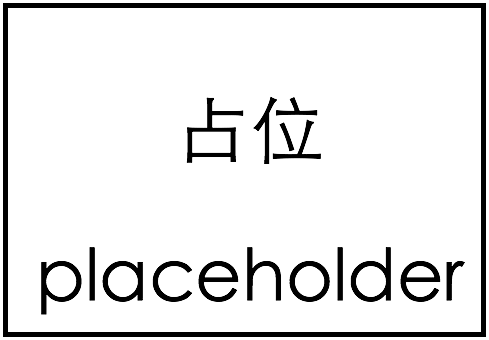
\includegraphics[width=0.5\linewidth]{figure/placeholder}
\fcaption{中文标题}{英文标题}[目录标题]
\label{fig:placeholder}
\end{figure}

\end{lstlisting}


\begin{figure*}[!htbp]
	\centering
	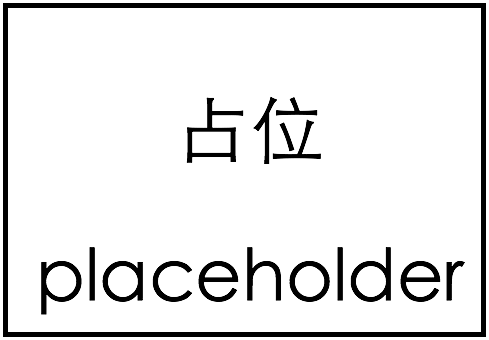
\includegraphics[width=0.5\linewidth]{figure/placeholder}
	\fcaption{中文标题}{英文标题}[目录标题]
	\label{fig:placeholder}
\end{figure*}

\section{表}

如表\ref{tab:table-example}所示,


\begin{lstlisting}[language=tex, label=lst:helloworld, caption=表-题注代码, numbers=left, basicstyle=\ttfamily]
\begin{figure}[!htbp]
\centering
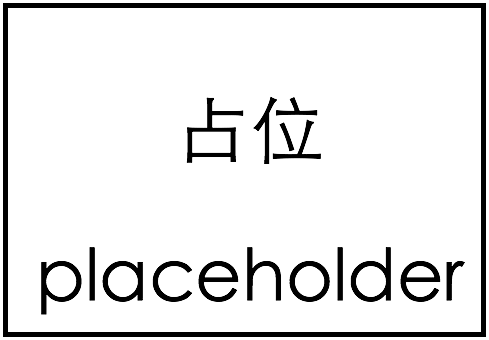
\includegraphics[width=0.5\linewidth]{figure/placeholder}
\fcaption{中文标题}{英文标题}[目录标题]
\label{fig:placeholder}
\end{figure}
\end{lstlisting}



\begin{table}[!htbp]
	\centering
	\tcaption{中文表标题}{引文表标题}[目录表标题]
	\label{tab:strength-of-hose}
	\begin{tabular}{@{\extracolsep{\fill}}>{\hspace{0.5cm}}clcccc}
		\toprule
		序号 &    规格     & \tabincell{c}{编织形式\\/mm×根 }& \tabincell{c}{实际\\爆破值/MPa }& \tabincell{c}{计算\\爆破值/MPa}& \tabincell{c}{偏差\\百分比}  \\ \midrule
		1  & Φ5(10.5MPa)  & Φ0.2×6  &   96.4    & 96.7          & 0.31\% \\
		2  & Φ8(10.5MPa)  & Φ0.3×5  &   83.5    & 83          & -0.60\% \\
		3  & Φ12(10.5MPa) & Φ0.3×6  &   63.5    & 66          & 3.94\%  \\
		4  & Φ16(5.0MPa)  & Φ0.3×6  &   47.1    & 51          & 8.28\% \\ \bottomrule
	\end{tabular} 
\end{table}  









%%==================================================
%% chapter03.tex for TJU Master Thesis
%% Encoding: UTF-8
%%==================================================

\chapter{ 代码详解}

\section{图}
\begin{lstlisting}[language=tex, label=lst:helloworld, caption=图-题注代码, numbers=left, basicstyle=\ttfamily]
\begin{figure}[!htbp]
\centering
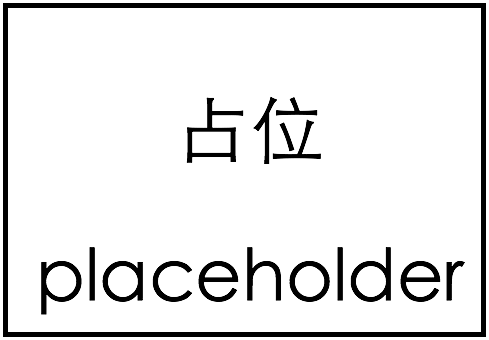
\includegraphics[width=0.5\linewidth]{figure/placeholder}
\fcaption{中文标题}{英文标题}[目录标题]
\label{fig:placeholder}
\end{figure}

\end{lstlisting}

\section{表}

\begin{lstlisting}[language=tex, label=lst:helloworld, caption=表-题注代码, numbers=left, basicstyle=\ttfamily]
\begin{table}[!htbp]
\centering
\tcaption{中文表标题}{英文表标题}[表格表标题]
\label{tab:table-example}
\begin{tabular*}{0.7\textwidth}{@{\extracolsep{\fill}}>{\hspace{0.5cm}}ccc}
\toprule
&  研究内容  &  研究方法 \\
\midrule
研究对象  &  研究内容  &  研究方法 \\
研究对象  &  研究内容  &  研究方法 \\
研究对象  &  研究内容  &  研究方法 \\
研究对象  &  研究内容  &  研究方法 \\
\bottomrule
\end{tabular*} 
\end{table}
\end{lstlisting}



%%==================================================
%% conclusion.tex for SJTU Master Thesis
%% based on CASthesis
%% modified by wei.jianwen@gmail.com
%% version: 0.3a
%% Encoding: UTF-8
%% last update: Dec 5th, 2010
%%==================================================

\chapter*{总结与展望\markboth{总结与展望}{}}
\addcontentsline{toc}{chapter}{总结与展望}



\vskip 3.8ex
\begin{flushleft}
	{\zihao{-3}\textbf{本文主要工作}}
\end{flushleft}
\vskip 1.2ex




\vskip 3.8ex
\begin{flushleft}
	{\zihao{-3}\textbf{本文主要贡献}}
\end{flushleft}
\vskip 1.2ex




\vskip 3.8ex
\begin{flushleft}
	{\zihao{-3}\textbf{下一步工作展望}}
\end{flushleft}
\vskip 1.2ex







\appendix	% 使用英文字母对附录编号,重新定义附录中的公式、图图表编号样式
\renewcommand\theequation{\Alph{chapter}--\arabic{equation}}	
\renewcommand\thefigure{\Alph{chapter}--\arabic{figure}}
\renewcommand\thetable{\Alph{chapter}--\arabic{table}}






\backmatter	% 文后无编号部分 

%% 参考资料

\bibliography{bib/preference}




%% 致谢、发表论文、参与项目、简历
%%==================================================
%% thanks.tex for SJTU Master Thesis
%% based on CASthesis
%% modified by wei.jianwen@gmail.com
%% version: 0.3a
%% Encoding: UTF-8
%% last update: Dec 5th, 2010
%%==================================================

\begin{thanks}
	
\zihao{4}\hangju{1}



\end{thanks}
 	%% 致谢
%%==================================================
%% pub.tex for SJTU Master Thesis
%% based on CASthesis
%% modified by wei.jianwen@gmail.com
%% version: 0.3a
%% Encoding: UTF-8
%% last update: Dec 5th, 2010
%%==================================================

\begin{publications}{99}



\item 

\item 

\item 
    
\end{publications}


	%% 发表论文
%%==================================================
%% projects.tex for SJTU Master Thesis
%% based on CASthesis
%% modified by wei.jianwen@gmail.com
%% version: 0.3a
%% Encoding: UTF-8
%% last update: Dec 5th, 2010
%%==================================================

\begin{projects}{99}
%
    \item 
%    
\end{projects}
  %% 参与的项目

\end{document}
